\documentclass{exam}
\newcommand{\splitcell}[2][c]{%
  \begin{tabular}[c]{@{}c@{}}\strut#2\strut\end{tabular}%
}
\usepackage{graphicx} % Required for inserting images
\usepackage{tikz}
\usepackage{listings} % Used for the programming coding 
\usepackage{geometry}
\geometry{margin=2cm} %used to fix a warning
\usepackage{xcolor} 
\usepackage{hyperref} %used for the refenrence to a subsection

\definecolor{codegreen}{rgb}{0,0.6,0}
\definecolor{codegray}{rgb}{0.5,0.5,0.5}
\definecolor{codepurple}{rgb}{0.58,0,0.82}
\definecolor{backcolour}{rgb}{0.95,0.95,0.92}

\lstdefinestyle{mystyle}{
    backgroundcolor=\color{backcolour},   
    commentstyle=\color{codegreen},
    keywordstyle=\color{magenta},
    numberstyle=\tiny\color{codegray},
    stringstyle=\color{codepurple},
    basicstyle=\ttfamily\footnotesize,
    breakatwhitespace=false,         
    breaklines=true,                 
    captionpos=b,                    
    keepspaces=true,                 
    numbers=none,                    
    numbersep=5pt,                  
    showspaces=false,                
    showstringspaces=false,
    showtabs=false,                  
    tabsize=2
}

\lstset{style=mystyle}



\begin{document}

\newcommand{\Exjobbsnummer}[1]{
	\begin{tikzpicture}[overlay, remember picture]
		\path (current page.north east) ++(-1,-1) node[below left] {{\small #1}};
	\end{tikzpicture}
}

\newcommand{\Examensjobbspoang}[1]{
	\begin{tikzpicture}[overlay, remember picture]
		\path (current page.north east) ++(-1,-1.5) node[below left] {{\normalsize \scshape Examensarbete #1 HP}};
	\end{tikzpicture}
}

\newcommand{\datum}[1]{
	\begin{tikzpicture}[overlay, remember picture]
		\path (current page.north east) ++(-1,-2.0) node[below left] {{\normalsize #1}};
	\end{tikzpicture}}

\newcommand{\storlitentitel}[2]{
\center
\rule[0.2cm]{13cm}{0.1cm}
{ \huge \bfseries #1}\\[0.4cm] % Title of your document
{\Large \slshape #2}\\[0.4cm]
\rule[0.2cm]{13cm}{0.1cm}\\[3cm]

}

\newcommand{\Namn}[2]{
	\begin{minipage}{0.5\textwidth}
		\normalsize
		\centering
		#1 \textsc{#2}\\
	\end{minipage}\\
}



\newcommand{\LoggaSwe}{
	\textsc{\Huge Computer Architecture and \\[0.3cm] Operating Systems}\\[0.3cm]
	
\includegraphics[scale=.06]{graphics/polito_logo_2021_blu.jpg.jpeg}\\[1.5cm]
}


% -----------------------------------------------
%           start titlepage
%------------------------------------------------
\begin{titlepage}
	\center 



 
	\Exjobbsnummer{Academic Year 2023/2024}	

 
	\LoggaSwe     


 
	\storlitentitel{\\Tutorial}{QEMU and FreeRTOS toolchain installation}    
 
        \Namn{Giorgio Fardo}{(s331003)}
	\Namn{Luca Ponzo}{(s323504)}
	\Namn{Michele Seira}{(s323595)}
        \Namn{Gianfranco Trad}{(s323713)}
	\vfill
\end{titlepage}

\pagebreak


\section{Installation of the toolchain for FreeRTOS with WSL on Windows}
Skip to the point \hyperref[1.2]{1.2} if the installation is done on a \textbf{GNU/Linux} OS, Adapt to the installed package manager.
\subsection{Ubuntu installation}
The first step to install \textbf{FreeRTOS} on your device is to set up the environment where it will run, and it can be done with:

\begin{lstlisting}
    wsl --install Ubuntu-22.04
\end{lstlisting}

A message will appear, which will ask to insert a \texttt{username} (without capital letter) and a \texttt{password} with a repetition of the same.

%\begin{figure}[h]
%    \centering
%    \includegraphics[width=0.90\textwidth]{test1.png}
%    \caption{possibile immagine da mettere}
%    \label{fig:riferimentoNelTestoNelCasoVogliaCitareLimmagine}
%\end{figure}
\subsection{Setting up the required packages}\label{1.2}
Using administrator privileges, you can add a new software repository to the \textbf{APT} (\texttt{Advanced Package Tool}) system used for package management in many \texttt{Debian}-based distributions, including \texttt{Ubuntu}. Specify the repository address, which in this case refers to a \textbf{PPA} (\texttt{Personal Package Archive}). \textbf{PPA}s are personal repositories that may contain additional software not found in the official \texttt{Ubuntu} repositories (to be verified; in this case, it pertains to updated versions of \texttt{Python}).
\begin{lstlisting}
    sudo add-apt-repository ppa:deadsnakes/ppa
\end{lstlisting}
Update the list of available packages from the software repositories configured in the system:
\begin{lstlisting}
    sudo apt update
\end{lstlisting}
Installing these packages provides the dependencies and libraries necessary to compile and run various types of software on your system:
\begin{lstlisting}
    sudo apt install git libglib2.0-dev libfdt-dev libpixman-1-dev zlib1g-dev ninja-build libncursesw5 libncurses5  python-is-python3 python3.8 build-essential libssl-dev zlib1g-dev libbz2-dev libreadline-dev libsqlite3-dev curl  libncursesw5-dev  xz-utils tk-dev libxml2-dev libxmlsec1-dev libffi-dev liblzma-dev 
\end{lstlisting}
Now download the file \texttt{get-pip.py} from the internet using the command:
\begin{lstlisting}
    wget  https://bootstrap.pypa.io/get-pip.py
\end{lstlisting}
Finally, install \textbf{pip} on \texttt{Python}'s system:
\begin{lstlisting}
    python get-pip.py
\end{lstlisting}
\subsection{Compilation and install of Qemu from source}
Create \textbf{Qemu}'s directory:
\begin{lstlisting}
    mkdir qemu
\end{lstlisting}
Go into the directory:
\begin{lstlisting}
    cd qemu
\end{lstlisting}
Now, download the compressed archive containing the source code for \texttt{version 8.2.0 Release Candidate 3} of \textbf{Qemu}, a processor emulator and virtualizer:
\begin{lstlisting}
    wget https://download.qemu.org/qemu-8.2.0-rc3.tar.xz
\end{lstlisting}
Decompress the recently installed repository:
\begin{lstlisting}
    tar xvJf qemu-8.2.0-rc3.tar.xz
\end{lstlisting}
Navigate to the \texttt{qemu-8.2.0-rc3} folder:
\begin{lstlisting}
    cd qemu-8.2.0-rc3
\end{lstlisting}
With this command, the configuration of the \textbf{Qemu}'s build process takes place, specifically targeting the \texttt{arm-softmmu} and \texttt{arm-linux-user} architecture:
\begin{lstlisting}
    ./configure --target-list=arm-softmmu, arm-linux-user
\end{lstlisting}
Compiling using 6 different cores can be achieved as follows; in the general case, check the system settings to determine the number of cores your device has, where you are executing this tutorial.
\begin{lstlisting}
    make -j6
\end{lstlisting}
\begin{figure}[h]
    \centering
    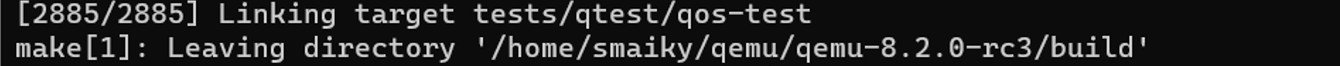
\includegraphics[width=0.90\textwidth]{graphics/make-j6.png}
    \caption{make-j6}
    \label{fig:riferimentoNelTestoNelCasoVogliaCitareLimmagine}
\end{figure}
Move the compiled files to the appropriate directories, creating links in the correct system directories:
\begin{lstlisting}
    sudo make install
\end{lstlisting}
\begin{figure}[h]
    \centering
    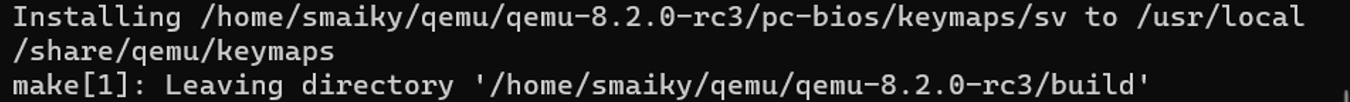
\includegraphics[width=0.90\textwidth]{graphics/make-install.png}
    \caption{make-install}
    \label{fig:riferimentoNelTestoNelCasoVogliaCitareLimmagine}
\end{figure}
After that, follow the below-mentioned path to enter the bin repository:
\begin{lstlisting}
    cd  /usr/local/bin 
\end{lstlisting}
Verify the version of the compiled \textbf{ARM} architecture-based system emulator from the previous steps:
\begin{lstlisting}
    ./qemu-system-arm --version
\end{lstlisting}
\begin{figure}[h]
    \centering
    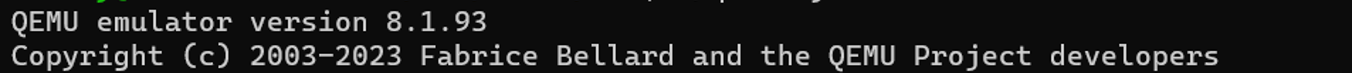
\includegraphics[width=0.90\textwidth]{graphics/qemu-system-arm-version.png}
    \caption{qemu-system-arm-version}
    \label{fig:riferimentoNelTestoNelCasoVogliaCitareLimmagine}
\end{figure}

\begin{lstlisting}
    cd
\end{lstlisting}
\subsection{ARM TOOLCHAIN}

Create a variable \textbf{ARM\_TOOLCHAIN\_VERSION} and assign it the version of the \texttt{ARM GNU Toolchain} extracted from the webpage \texttt{https://developer.arm.com/downloads/-/arm-gnu-toolchain-downloads}:

\begin{lstlisting}
    ARM_TOOLCHAIN_VERSION=$(curl -s https://developer.arm.com/downloads/-/arm-gnu-toolchain-downloads | grep -Po '<h4>Version \K.+(?=</h4>)')    
\end{lstlisting}
With this command, you will download the zip file \texttt{gcc-arm-none-eabi}, which contains the version tied to the \texttt{bash} variable defined in the previous command:
\begin{lstlisting}
    curl -Lo gcc-arm-none-eabi.tar.xz https://developer.arm.com/-/media/Files/downloads/gnu/${ARM_TOOLCHAIN_VERSION}/binrel/arm-gnu-toolchain-${ARM_TOOLCHAIN_VERSION}-x86_64-arm-none-eabi.tar.xz
\end{lstlisting}
Create the directory:
\begin{lstlisting}
    sudo mkdir /opt/gcc-arm-none-eabi
\end{lstlisting}
Now, with administrator privileges, extract the contents of the \texttt{gcc-arm-none-eabi.tar.xz} archive and place it in the specified directory:
\begin{lstlisting}
    sudo tar xf gcc-arm-none-eabi.tar.xz --strip-components=1 -C /opt/gcc-arm-none-eabi
\end{lstlisting}
With this command, you add the specified path to the \texttt{PATH}, ensuring that the \textbf{GNU ARM Toolchain} executables are globally available in the system by appending a string to the specified file.
\begin{lstlisting}
    echo 'export PATH=$PATH:/opt/gcc-arm-none-eabi/bin' | sudo tee -a /etc/profile.d/gcc-arm-none-eabi.sh
\end{lstlisting}
When you execute this command, the settings and environment variables defined in the previous commands in "\texttt{etc/profile}" become immediate and available in the current session.
\begin{lstlisting}
    source /etc/profile
\end{lstlisting}
To check the version of \textbf{arm-none-eabi-gcc}
\begin{lstlisting}
    arm-none-eabi-gcc  --version 
\end{lstlisting}
\begin{figure}[h]
    \centering
    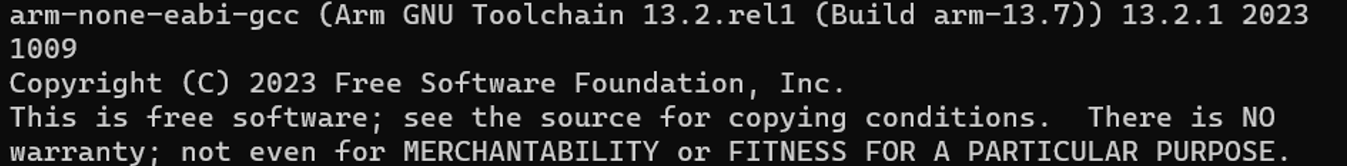
\includegraphics[width=0.90\textwidth]{graphics/arm-none-eabi-gcc-version.png}
    \caption{arm-none-eabi-gcc  --version}
    \label{fig:riferimentoNelTestoNelCasoVogliaCitareLimmagine}
\end{figure}
To check the version of \textbf{arm-none-eabi-gdb}
\begin{lstlisting}
    arm-none-eabi-gdb --version 
\end{lstlisting}
\begin{figure}[h]
    \centering
    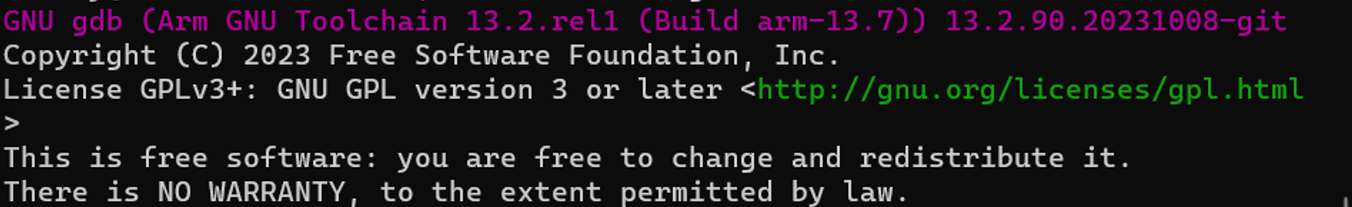
\includegraphics[width=0.90\textwidth]{graphics/arm-none-eabi-gdb-version.png}
    \caption{arm-none-eabi-gdb --version}
    \label{fig:riferimentoNelTestoNelCasoVogliaCitareLimmagine}
\end{figure}
\subsection{FreeRTOS download}
To set the Git configuration "\texttt{core.symlinks}" to true, making Git treat symbolic links as such:
\begin{lstlisting}
    git config --global core.symlinks true 
\end{lstlisting}
The command used to clone an existing Git repository, in this case, cloning the FreeRTOS repository from the \textbf{GitHub} site:
\begin{lstlisting}
    git clone https://github.com/FreeRTOS/FreeRTOS.git --recurse-submodules
\end{lstlisting}
\begin{figure}[h]
    \centering
    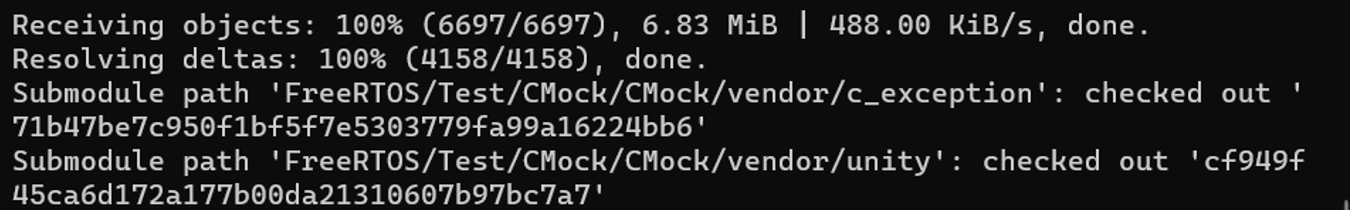
\includegraphics[width=0.90\textwidth]{graphics/git-clone-freertos.png}
    \caption{qemu-system-arm-version}
    \label{fig:riferimentoNelTestoNelCasoVogliaCitareLimmagine}
\end{figure}

\subsection{Debugger utilization}
Now navigate to the directory:
\begin{lstlisting}
    cd FreeRTOS/FreeRTOS/Demo/CORTEX_MPS2_QEMU_IAR_GCC   
\end{lstlisting}
Enter to the file \texttt{main.c}
\begin{lstlisting}
    nano main.c
\end{lstlisting}
Check if the variable in the file is set like below
\begin{lstlisting}
    #define mainCREATE_SIMPLE_BLINKY_DEMO_ONLY      1
\end{lstlisting}
Exit from the file and go into this directory
\begin{lstlisting}
    Cd build/gcc
\end{lstlisting}
Compilation as before
\begin{lstlisting}
    Make -j6
\end{lstlisting}
This command starts a \textbf{QEMU} simulation of an \textbf{ARM Cortex-M3 system}, loads a specified kernel image, disables the graphical interface, redirects serial output to the terminal, and pauses the simulation, waiting for a debugger to connect.
\begin{lstlisting}
    qemu-system-arm -machine mps2-an385 -cpu cortex-m3 -kernel ./output/RTOSDemo.out -monitor none -nographic -serial stdio -s -S
\end{lstlisting}
If you open another terminal to interact with the newly created virtual machine and it gives you two options, such as the ability to continue with "pow", you are likely interacting with a \textbf{QEMU monitor}.
\begin{lstlisting}
    wsl 
\end{lstlisting}

\begin{lstlisting}
    cd --
\end{lstlisting}
Enter to the output directory.
\begin{lstlisting}
    cd  FreeRTOS/FreeRTOS/Demo/CORTEX_MPS2_QEMU_IAR_GCC/build/gcc/output
\end{lstlisting}
This command launches the \textbf{ARM} version of the \texttt{GNU Debugger (GDB)} and loads the specific binary file ('\texttt{RTOSDemo.out}) for debugging.
\begin{lstlisting}
    arm-none-eabi-gdb RTOSDemo.out
\end{lstlisting}
This command in \textbf{GDB} establishes a remote connection to a target using the \textbf{GDB} Remote Serial Protocol. This is commonly used when debugging a program running on a different machine.
\begin{lstlisting}
    target remote localhost:1234
\end{lstlisting}



























\setcounter{enumi}{0}

\section{Installation of the toolchain for FreeRTOS natively on Windows}

In the following steps there is a guide on how to setup \textbf{FreeRTOS} and \textbf{QEMU} on windows and run a simple demo to ensure everything is working.
To go forward with the installation keep in mind that there are different choices as an \textbf{SOC} to emulate, in this guide it is used an \textbf{mps-an385}, meaning that it will be explained how to setup an ARM debugger. If you want to install FreeRTOS and Qemu but decide to go with another architecture please refer to \href{https://www.freertos.org/a00090.html}{the official FreeRTOS documentation}.

\subsection{QEMU}

To download QEMU on windows refer to \href{https://www.qemu.org/download/#windows}{the official QEMU documentation} and download the right executable for your OS architecture; after that just open the executable, if it opens just skip chapter \textbf{2.1} (Command prompt execution) and go for \textbf{2.2} (Standard execution).

 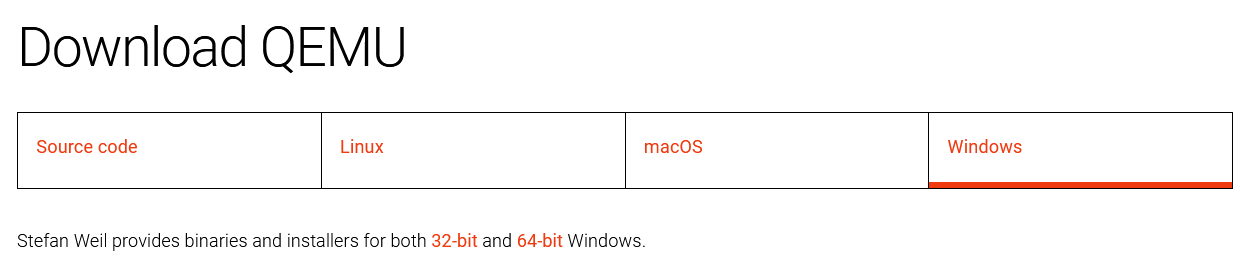
\includegraphics[width=\textwidth]{1a}

 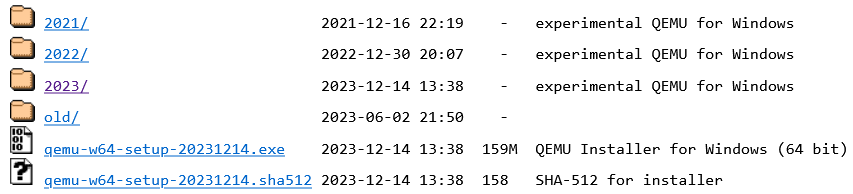
\includegraphics[width=\textwidth]{1b}

\subsubsection {Command prompt execution} 
\begin{enumerate}
\item open the command prompt as an administrator
\item go to the directory of the QEMU installer
\item type the name of the QEMU installer in the command prompt, it should open now
\item go forward with the \textbf{Standard installation}
\end{enumerate}


 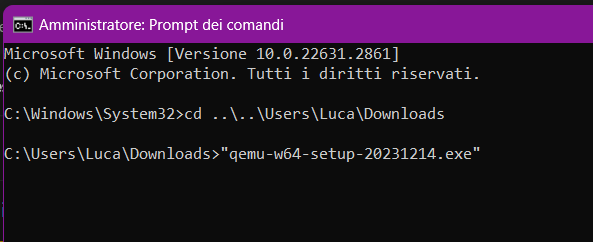
\includegraphics[width=\textwidth]{1c}

\subsubsection{Standard execution} 

Just press forward and keep in mind the location in which you decide to install qemu, it will become handy sooner.

\subsubsection {Add to environment path} 
After the installation it's needed to add QEMU to the system PATH, you can do it by searching "environment variables" and clicking on the first result, when the window opens:

\begin{enumerate}
    \item search the item with the text PATH on the upper section of the window 
     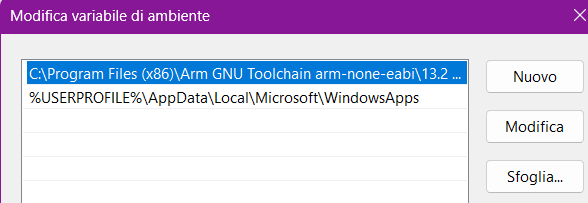
\includegraphics[width=\textwidth]{1e}
    \item click on edit
    \item add a new entry and put the path where qemu is installed (default is \textbf{C:\textbackslash Program Files\textbackslash qemu})
    
    \includegraphics[width=\textwidth]{1f}
    
    \item click ok on all the windows opened
\end{enumerate}

\subsection{MAKE}

After QEMU we need some tools to build our FreeRTOS instance, in this guide it will be used 
\begin{lstlisting}
    make
\end{lstlisting}.
Make can be downloaded \href{https://gnuwin32.sourceforge.net/packages/make.htms}{from this source}, after choosing the right OS you can start to download it.

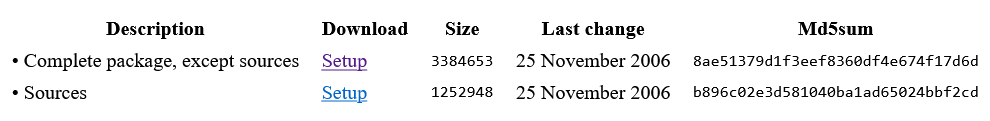
\includegraphics[width=\textwidth]{2a}

\subsection{Installation} 
    \begin{enumerate}
        \item follow the installation process, you can just keep forward, the only thing to remember is that you need to \textbf{save the installation path}.

        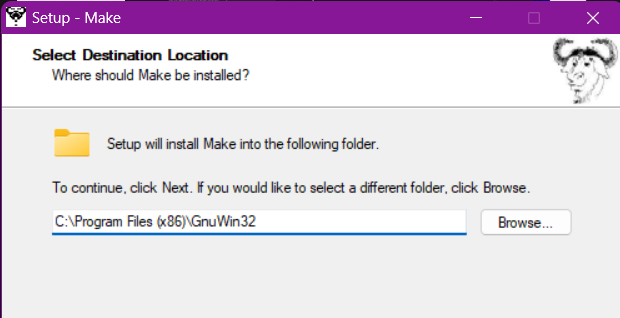
\includegraphics[width=\textwidth]{2b}

        \item after the installation is concluded add make to the system PATH, just follow point \textbf{2.3} but change the directory to \textit{make-dir}\textbackslash bin, as an example, if you install make in the same path as the image above you'll need to add to the PATH the directory \textbf{C:\textbackslash Program Files(x86)\textbackslash GnuWin32\textbackslash bin},

        \item check that make is properly installed by typing 
\begin{lstlisting}
    make -v 
\end{lstlisting} 
        on a command prompt window \textbf{freshly opened}, if the prompt gives an error make sure the PATH you set is correct and then try again.
        
    \end{enumerate}

\subsection{ARM Toolchain}

Since we are using an ARM SOC we'll need a matching compiler and debugger, we can download them from \href{https://developer.arm.com/downloads/-/arm-gnu-toolchain-downloads}{the official website}

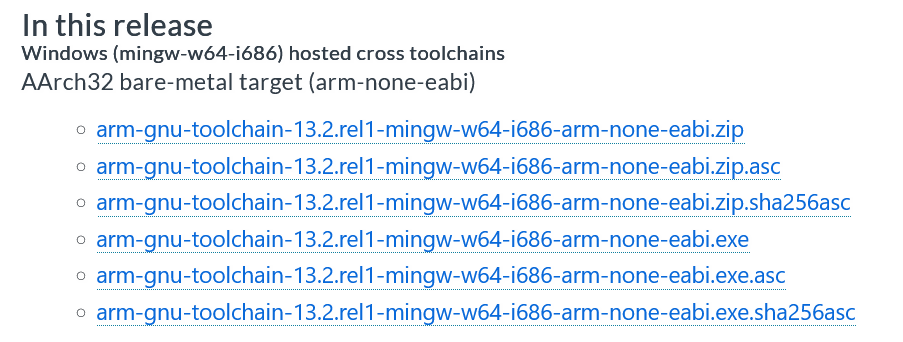
\includegraphics[width=\textwidth]{3a}

\subsubsection{Installation} 
As for the arm toolchain, life is easier, just keep sure to check the box \textbf{Add path to environment variable} in the end, if you didn't, you'll need to refer again to \textbf{2.3} and add \textit{arm-toolachain-dir}\textbackslash bin to the PATH manually.

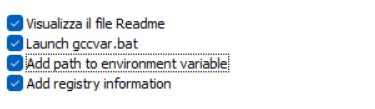
\includegraphics[width=\textwidth]{3b}

\subsection{FreeRTOS}

After having installed all the necessary tools we can download and install FreeRTOS. First thing first we'll need to download the System, in this case is a little more complex than before.

\subsubsection{Download}
    \begin{enumerate}
        \item open a command prompt and go in the folder you want to keep FreeRTOS
        \item enable git submodules by typing
\begin{lstlisting}
    git config --global core.symlinks true
\end{lstlisting}
        \item clone the repository by typing
\begin{lstlisting}
    git clone https://github.com/FreeRTOS/FreeRTOS.git --recurse submodules
\end{lstlisting}
    \end{enumerate}

\subsubsection{Installation}
    \begin{enumerate}
        \item go to \textbf{\textit{FreeRTOS-dir}\textbackslash FreeRTOS\textbackslash Demo\textbackslash CORTEX\textunderscore MPS2\textunderscore QEMU\textunderscore IAR\textunderscore GCC\textbackslash build\textbackslash gcc}
        \item type \textbf{make}
        \item if all the steps above went fine, you should have the file \textbf{.\textbackslash output\textbackslash RTOSDemo.out}
        \item if you want to run the blink demo, edit \textbf{.\textbackslash output\textbackslash main.o} and make sure the line \textbf{mainCREATE\textunderscore SIMPLE\textunderscore BLINKY\textunderscore DEMO\textunderscore ONLY} is defined to \textbf{1}.

        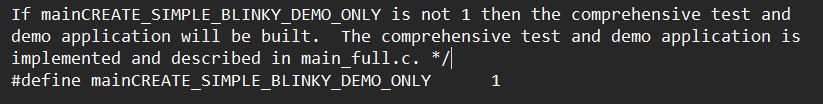
\includegraphics[width=\textwidth]{4}
    \end{enumerate}
    
\subsubsection{Starting FreeRTOS}
If the installation procere is concluded, you should be able to run FreeRTOS in QEMU by just typing one single command:
\begin{lstlisting}
    qemu-system-arm -machine mps2-an385 -cpu cortex-m3 -kernel <FreeRTOS dir>\FreeRTOS\Demo\CORTEX_MPS2_QEMU_IAR_GCC\build\gcc\output\RTOSDemo.out -monitor stdio -s -S
\end{lstlisting}


\subsubsection{Debugger utilization}
    \begin{enumerate}
        \item open a new command prompt and go to the directory of RTOSDemo.out
        \item type the command 
\begin{lstlisting}
    arm-none-eabi-gdb RTOSDemo.out
\end{lstlisting}
        \item connect to the qemu instance, it should be opened in the default port: \textbf{1234}, you can do that by typing 
\begin{lstlisting}
    target remote localhost:1234
\end{lstlisting}
        \item if you type \textbf{continue} the blinky demo will start.
    \end{enumerate}





\end{document}
